\chapter{Conclusion and Future Recommendations}

\section{Lesson Learnt / Outcome}

\subsection{Home Page}
The Home Page serves as the heart of our platform. It provides users with a friendly and intuitive starting point, presenting essential navigation options, important announcements, and recent activity highlights. With its carefully crafted layout, users can effortlessly explore different sections, ensuring a seamless and engaging experience that keeps them informed and connected to the latest updates and content.
\begin{figure}[ht]
    \centering
    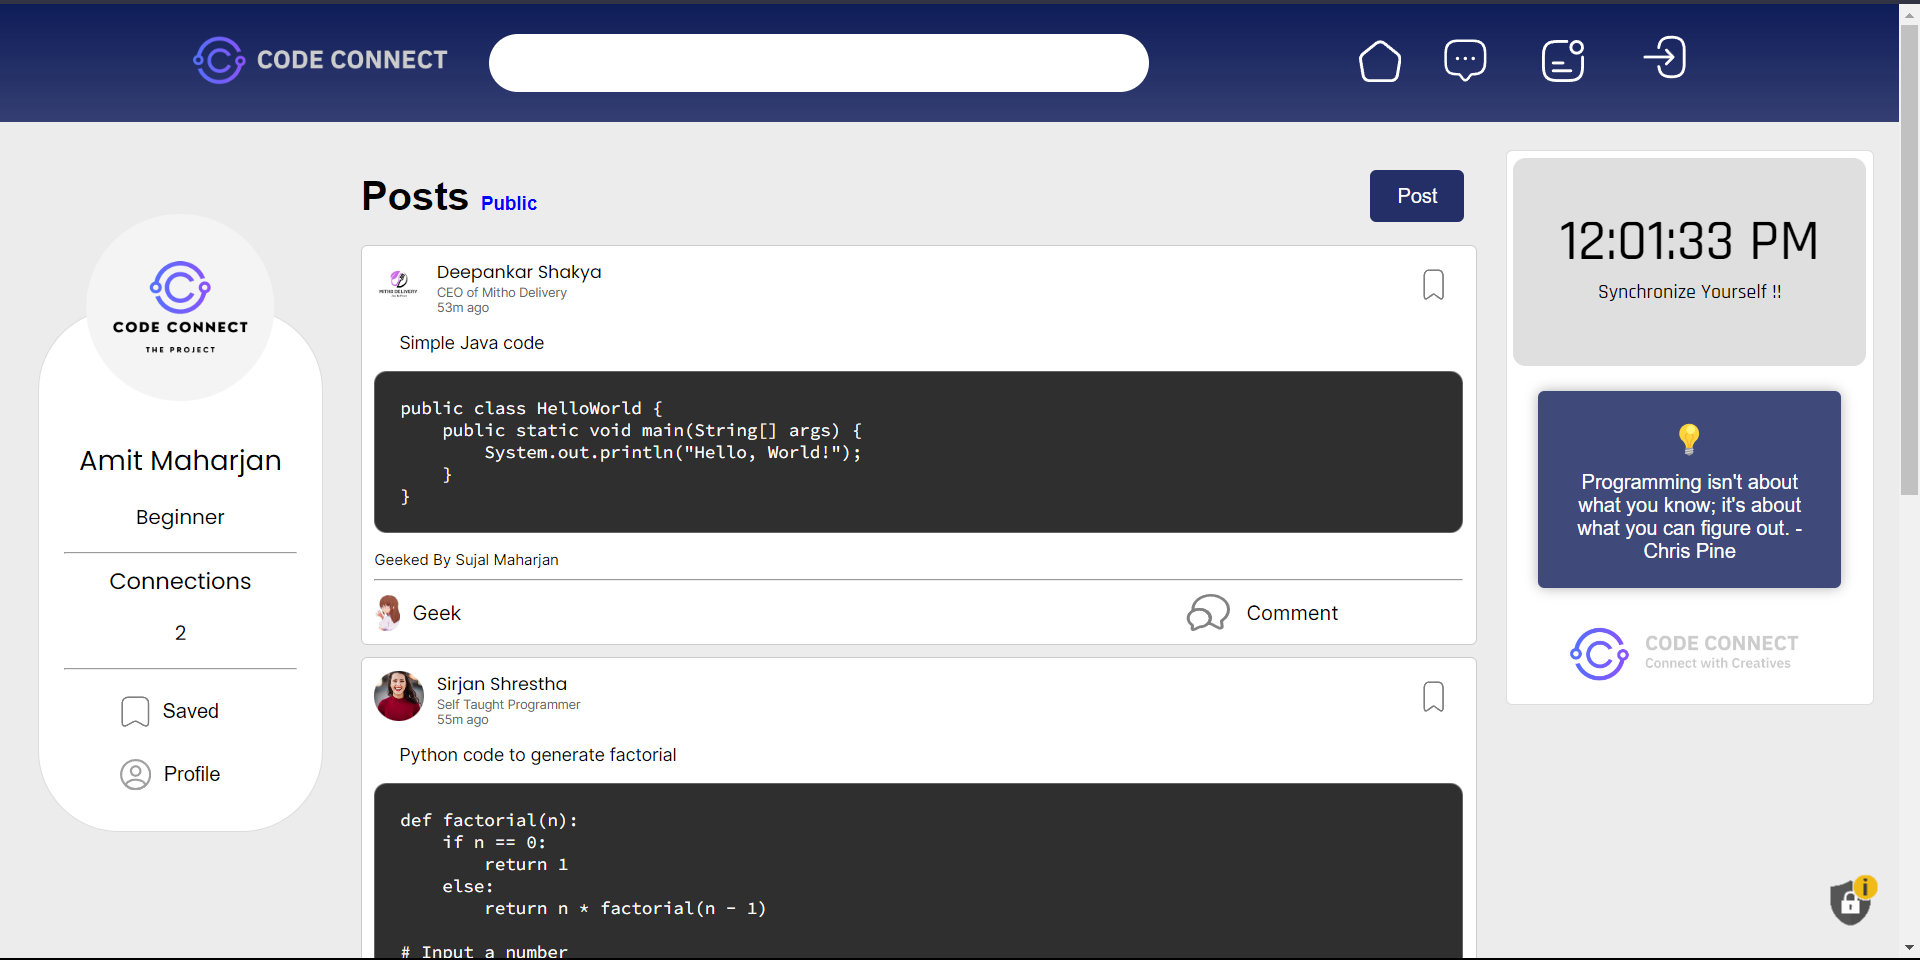
\includegraphics[width=1\textwidth]{Outcome-ss/homepage.png}
    \caption{Home Page.}
    \label{fig:Home Page}
\end{figure}

\subsection{Geek}
The image illustrates what happens when a user clicks on "geek." It's similar to how "like" button used to show that user enjoy something. Pressing "geek" is like giving a thumbs up, showing that the user finds the content interesting or cool, much like using a "like" button.
\begin{figure}[ht]
    \centering
    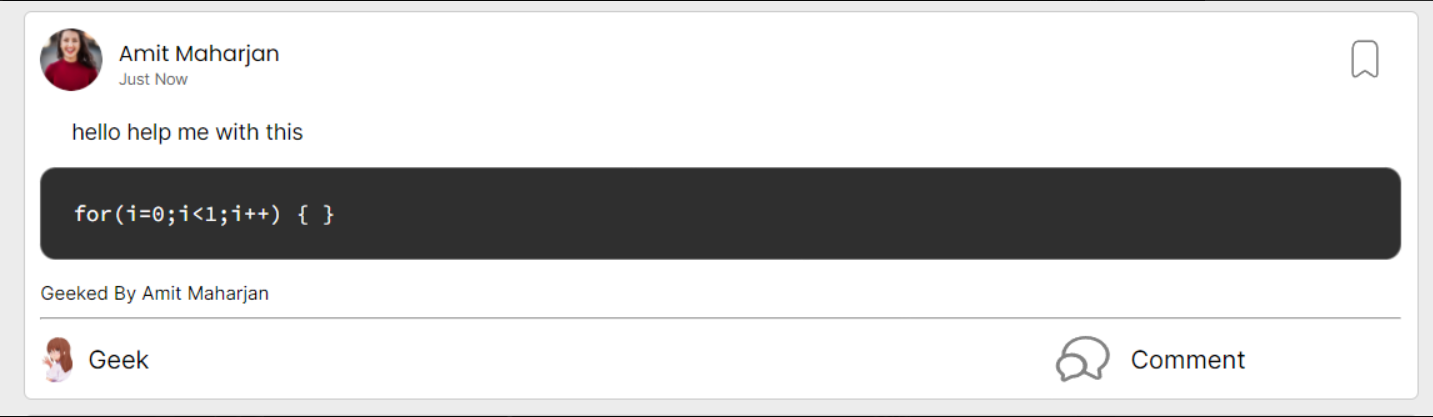
\includegraphics[width=0.9\textwidth]{Outcome-ss/geek.png}
    \caption{Geek.}
    \label{fig:Geek}
\end{figure}
\newpage
\subsection{Un-Geek}
In the picture, you can see what happens when a user clicks "un-geek." It's like taking back a previous action, kind of like when you change your mind about liking something. Just as you can "unlike" by using a "dislike" button, "un-geek" lets you remove the interest or approval you showed earlier with the "geek" feature.
\begin{figure}[H]
    \centering
    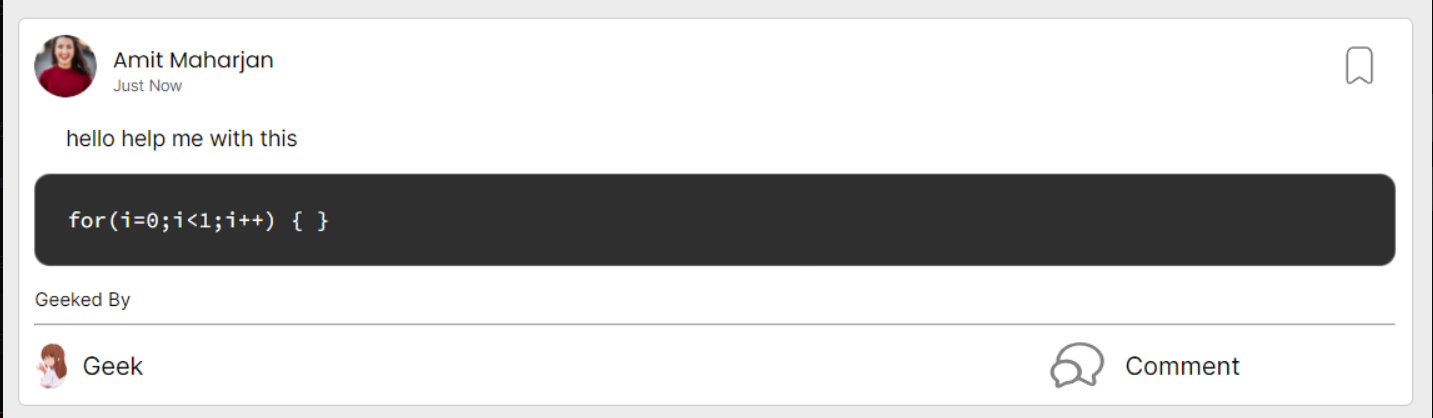
\includegraphics[width=0.9\textwidth]{Outcome-ss/ungeek.png}
    \caption{Un-Geek.}
    \label{fig:Un-Geek}
\end{figure}

\subsection{Profile}
The image displayed portrays the user profile within Code Connect. This profile presents a snapshot of the user's presence on the platform, offering insights into their activities, interests, and possibly their expertise. By showcasing key information, the profile facilitates connections and understanding among users, fostering a sense of community and collaboration within the Code Connect ecosystem.
\begin{figure}[ht]
    \centering
    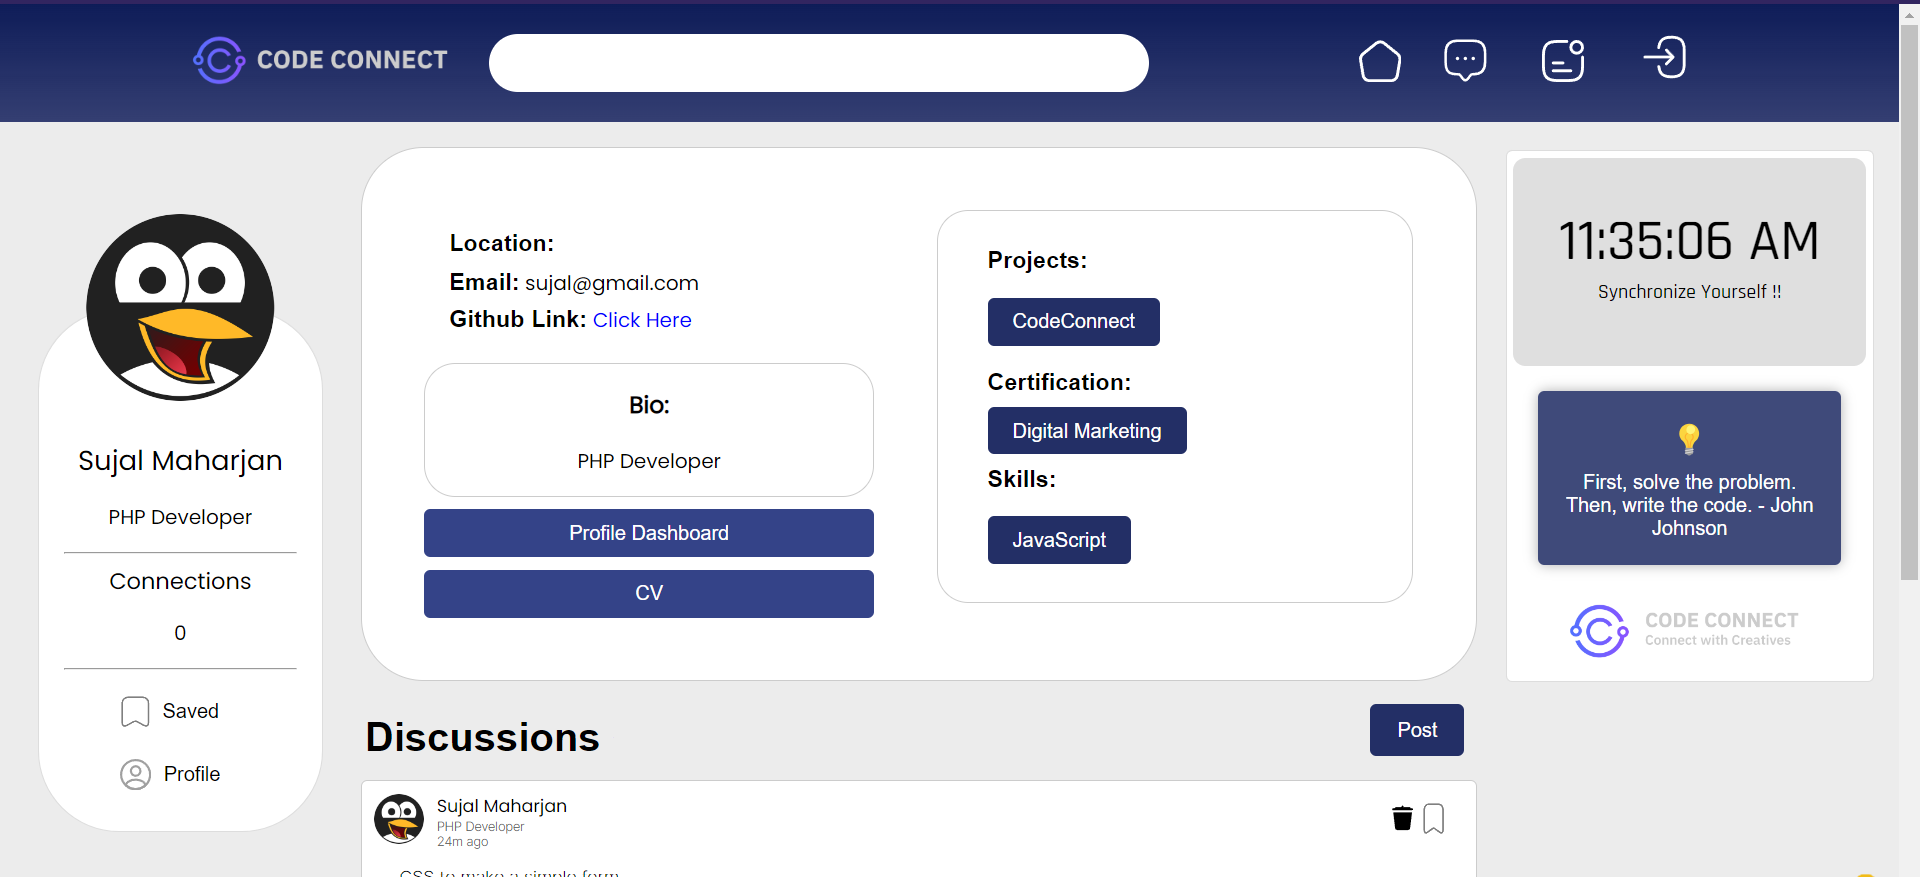
\includegraphics[width=1\textwidth]{Outcome-ss/self-profile.png}
    \caption{Profile.}
    \label{fig:Profile}
\end{figure}
\newpage
\subsection{Messenger}
In the picture, you can see the messaging part of Code Connect. It's like a chat where users can talk in real-time. This helps users easily share information, talk about projects, and ask for help within the Code Connect community. This messaging feature makes it simple for users to connect, share ideas, and work together on coding stuff.
\begin{figure}[ht]
    \centering
    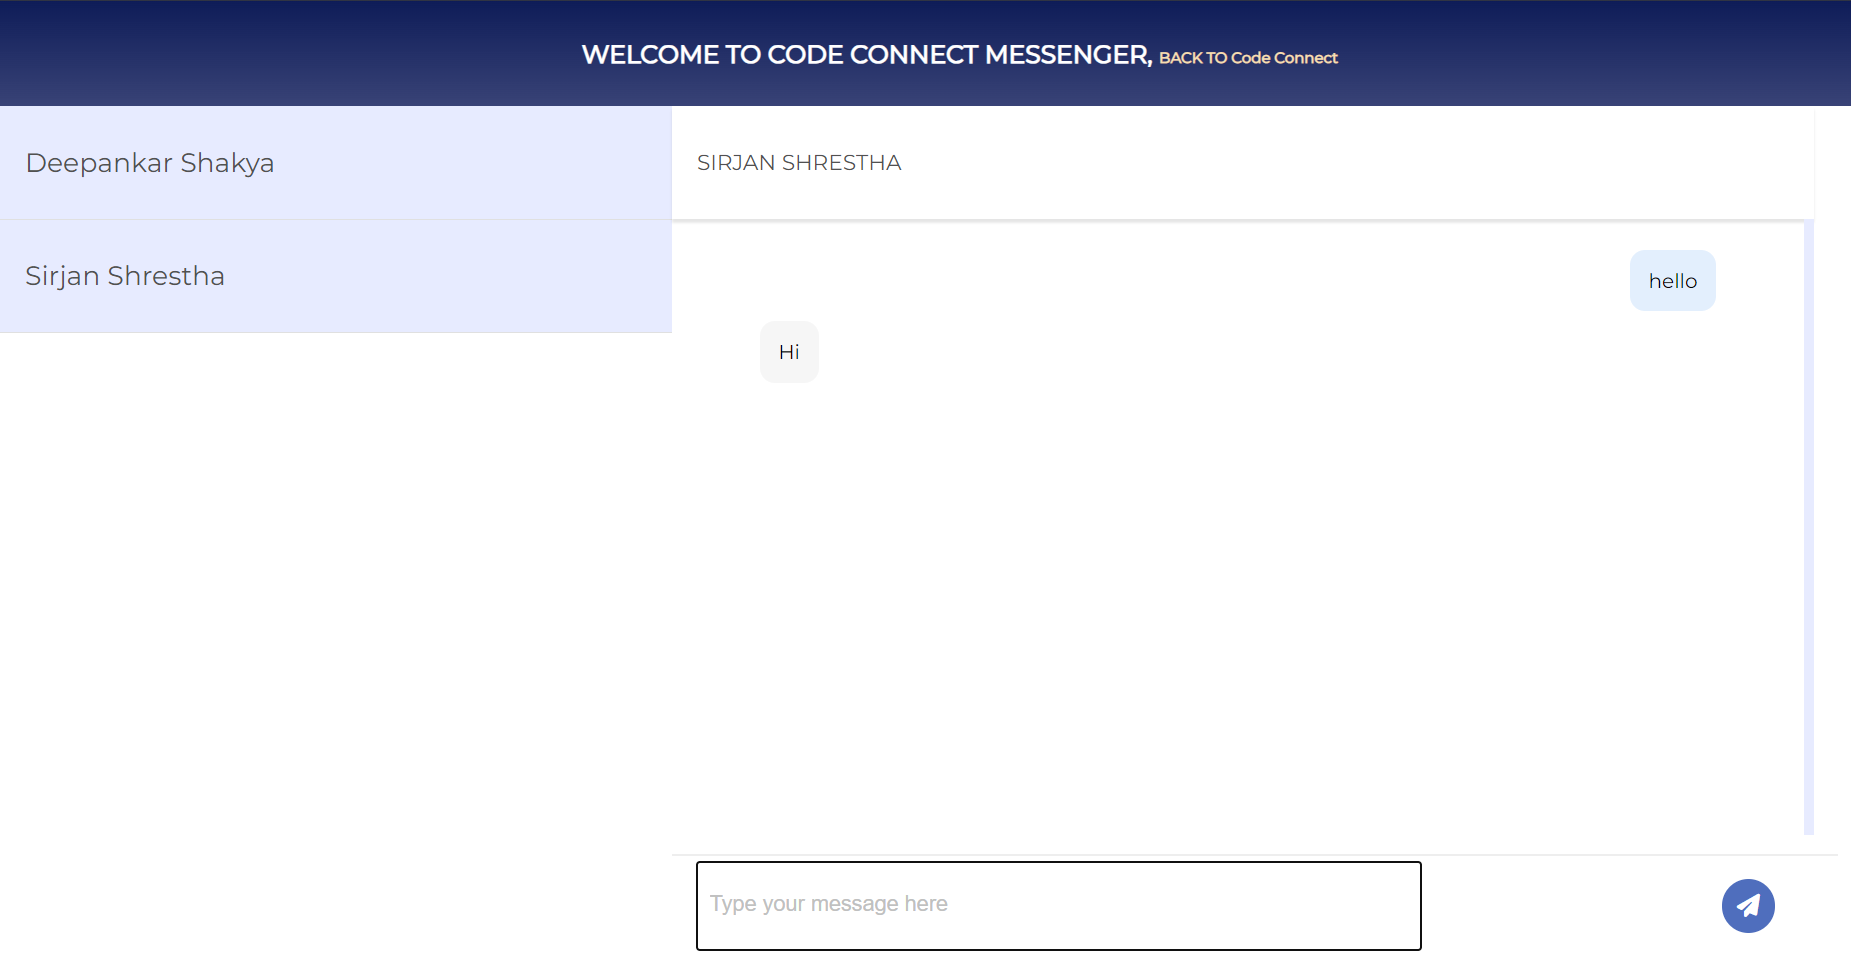
\includegraphics[width=1\textwidth]{Outcome-ss/messenger-full-block.png}
    \caption{Messenger.}
    \label{fig:Messenger}
\end{figure}

\subsection{Search}
"Code Connect" features an efficient search function where users can enter partial user names. As they type, the system dynamically suggests relevant user names that start with the typed letters. These suggestions appear in real-time below the search bar, aiding users in quickly finding and connecting with others. The process enhances user experience by providing instant, tailored recommendations based on the input, streamlining the connection process within the application.
\begin{figure}[ht]
    \centering
    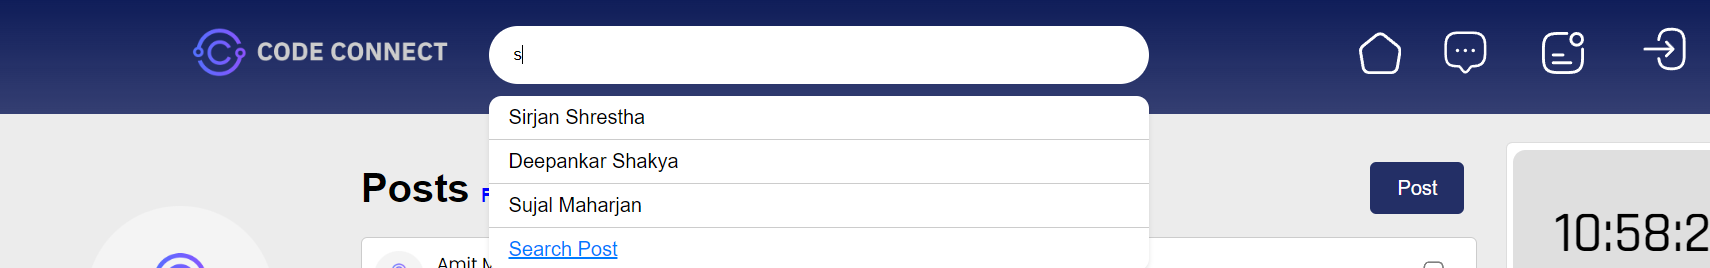
\includegraphics[width=0.9\textwidth]{Outcome-ss/search-bar.png}
    \caption{Search.}
    \label{fig:Search}
\end{figure}

\subsection{Notification}
The image displayed below showcases the notification feature of Code Connect. This tool is designed to keep users informed about important updates and activities. Notifications ensure that users stay in the loop about significant interactions or changes within the platform. By providing these alerts, the notification system enhances user engagement and helps users effectively stay connected and engaged within the Code Connect community.
\begin{figure}[ht]
    \centering
    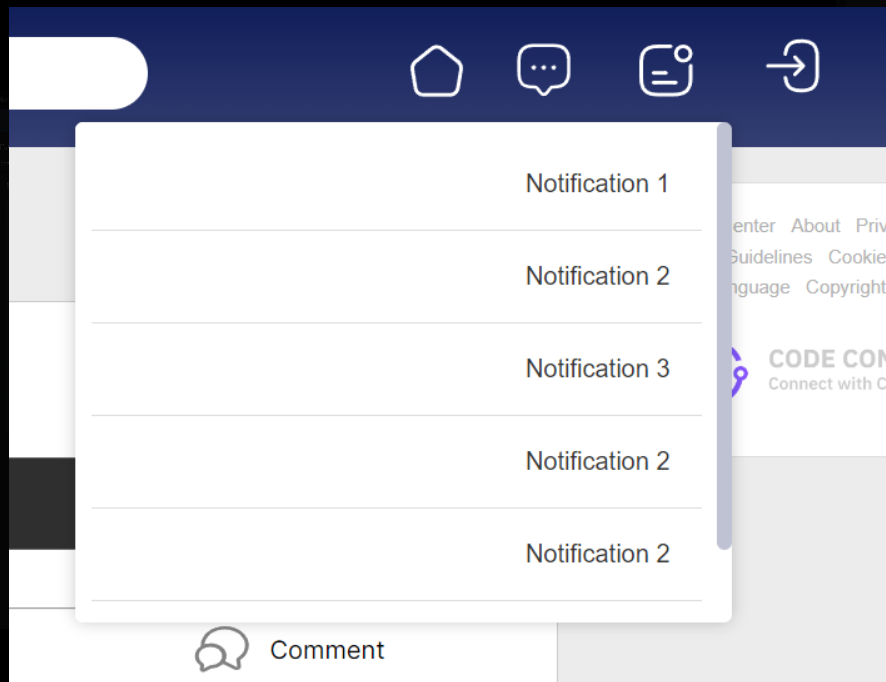
\includegraphics[width=0.5\textwidth]{Outcome-ss/notification.png}
    \caption{Notification.}
    \label{fig:Notification}
\end{figure}

\subsection{Post}
In the picture, you can see how you can make posts in Code Connect. It's like writing a message where you can share text and pieces of code. This helps you start conversations, show your coding work, and get advice from other users. It's a way to work together and learn from each other in Code Connect.
\begin{figure}[ht]
    \centering
    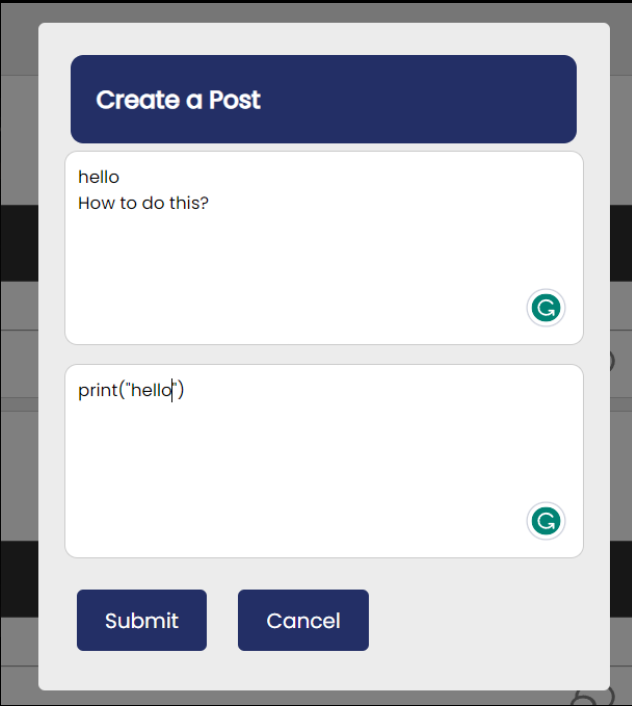
\includegraphics[width=0.5\textwidth]{Outcome-ss/post.png}
    \caption{Post.}
    \label{fig:Post}
\end{figure}

\subsection{Save Post}
The picture below shows how the user can re-visit the posts that is already saved.
\begin{figure}[ht]
    \centering
    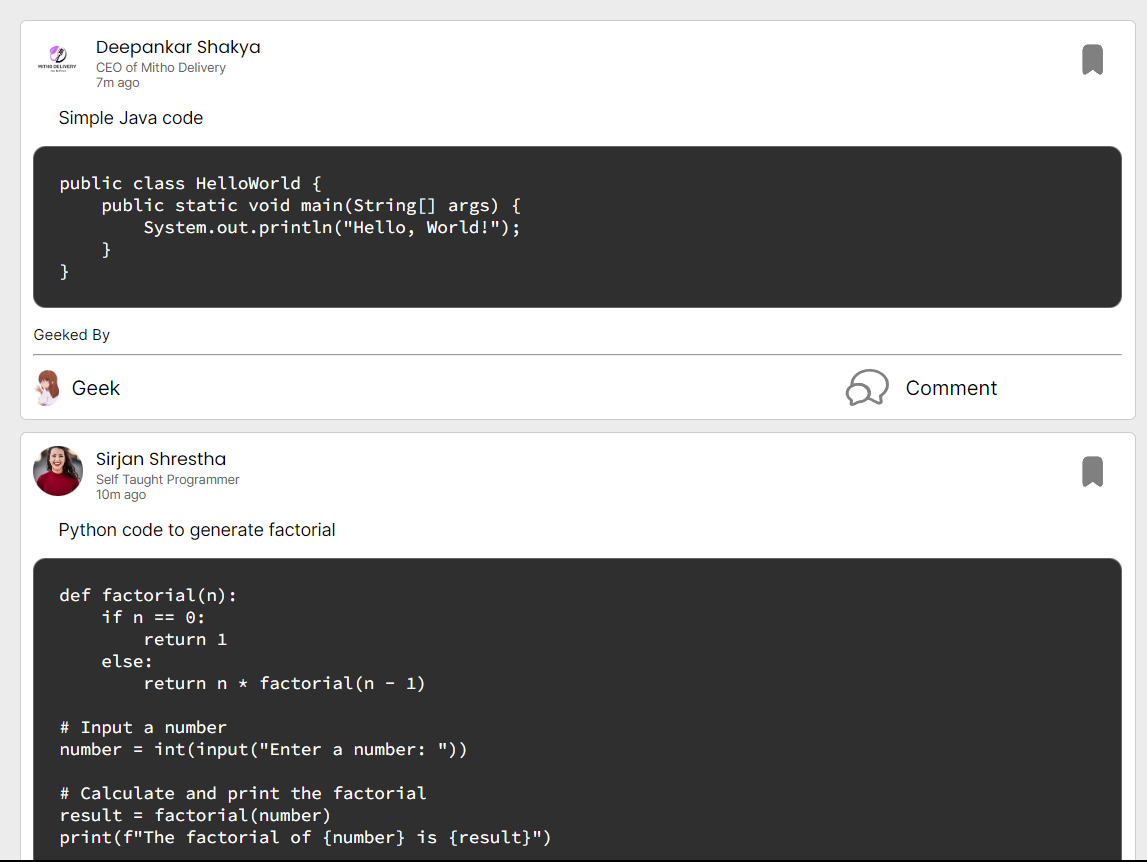
\includegraphics[width=0.5\textwidth]{Outcome-ss/saved-posts-list.png}
    \caption{Save post}
    \label{fig:Save Post}
\end{figure}

\subsection{Friends Posts}
This picture demonstrate how the user can manage posts so that it only shows the posts from the user's friend.
\begin{figure}[H]
    \centering
    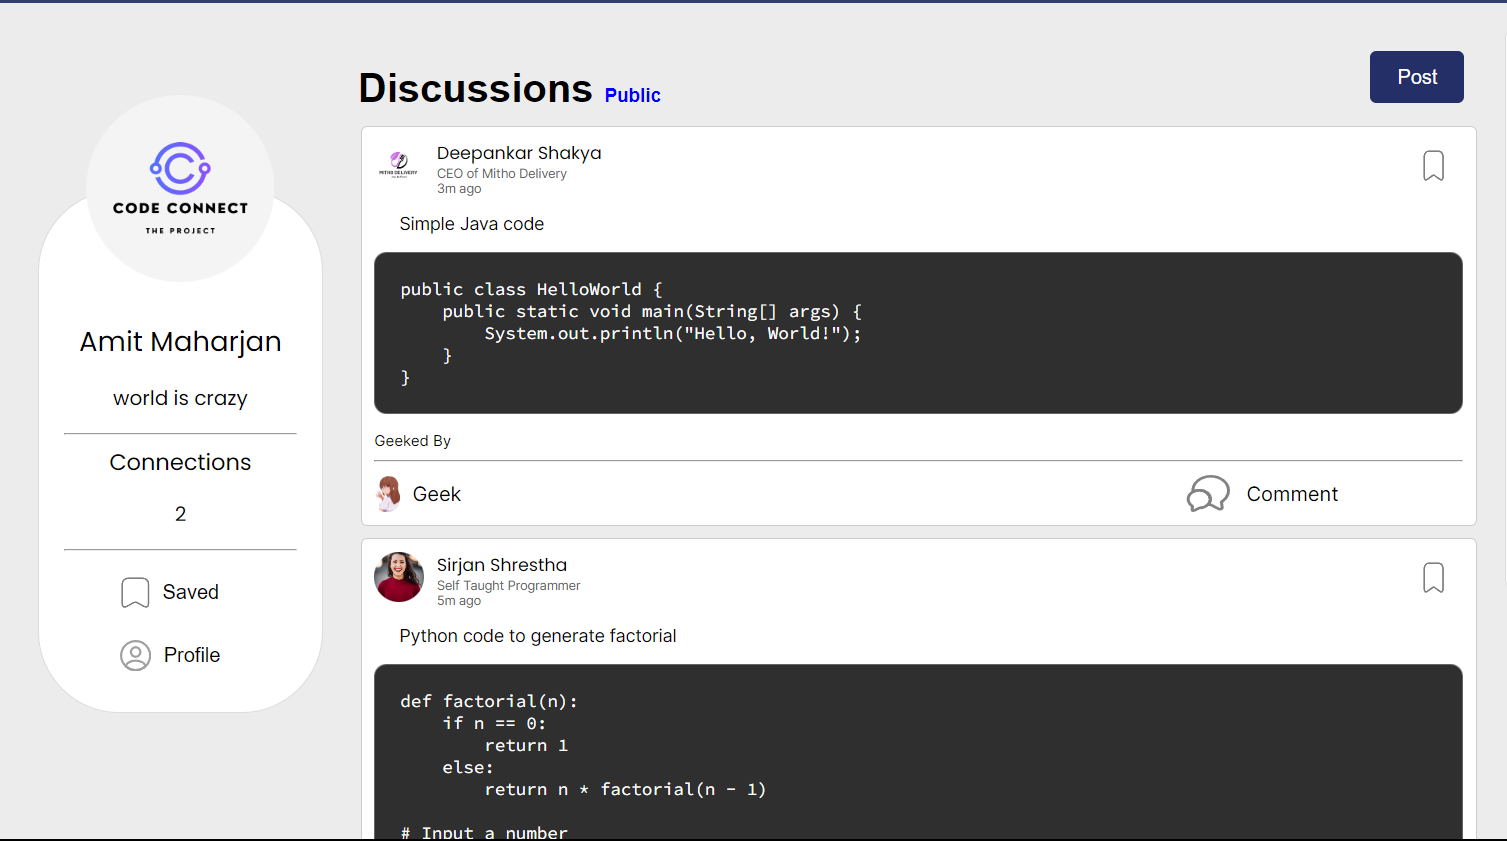
\includegraphics[width=0.5\textwidth]{Outcome-ss/friends-posts.png}
    \caption{Friends posts}
    \label{fig:Friends posts}
\end{figure}

\subsection{Public Posts}
This picture demonstrate how the user can manage posts so that it shows the posts of all the users (i.e Public).
\begin{figure}[H]
    \centering
    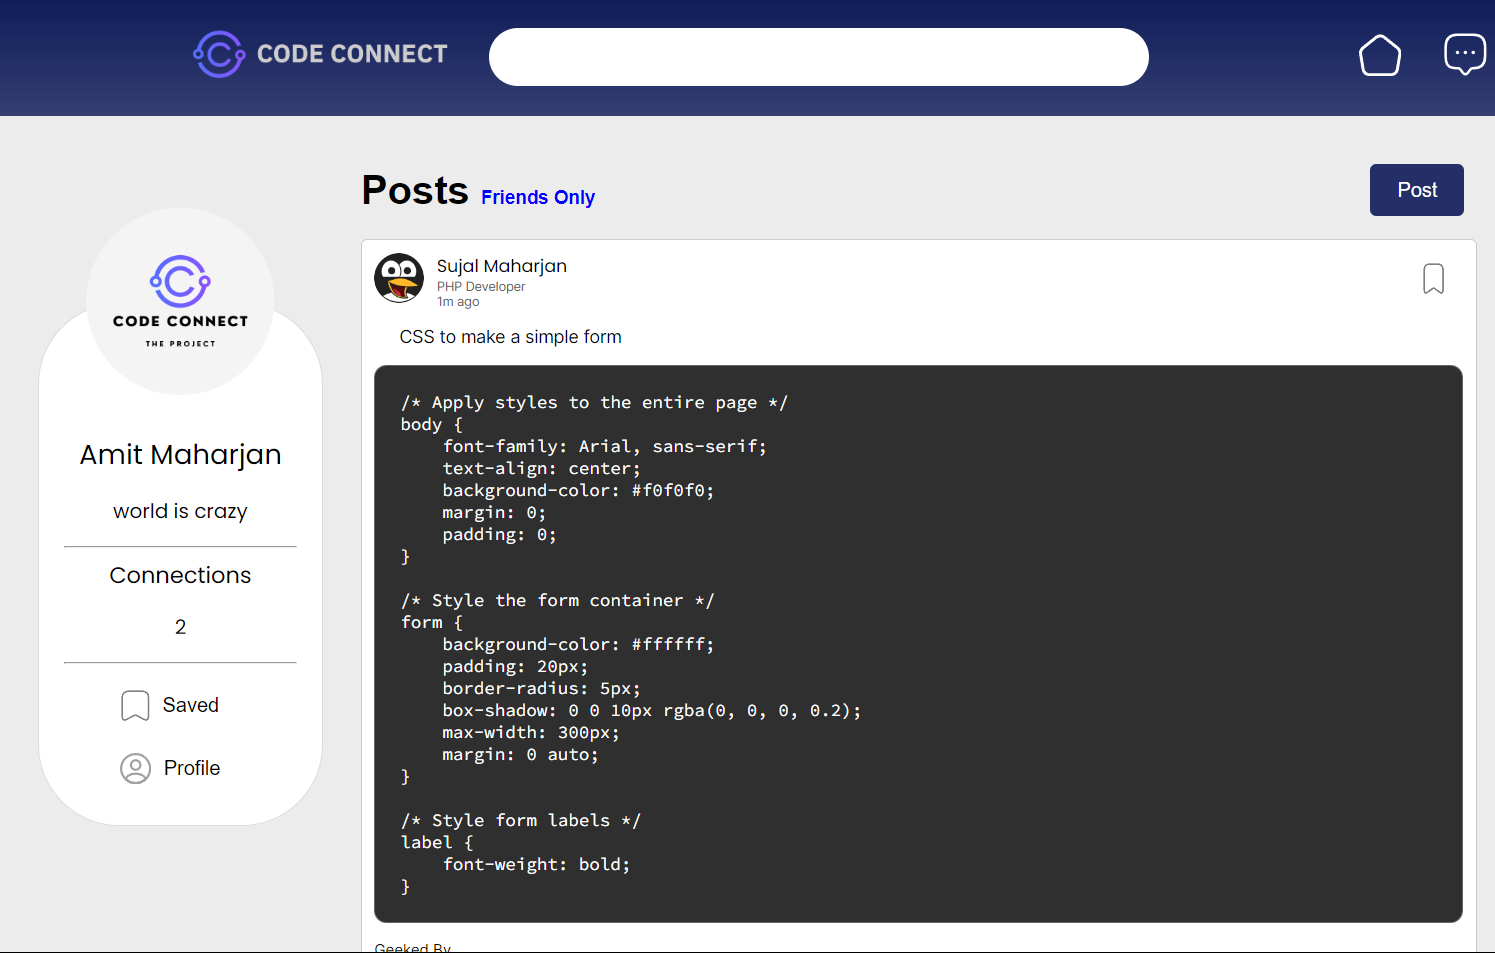
\includegraphics[width=0.5\textwidth]{Outcome-ss/public-posts.png}
    \caption{Public posts}
    \label{fig:Public posts}
\end{figure}
\subsection{Profile of other Users}
In the image below, you can see the profile section of other users. This section provides insights into their details, interests, and activities within the platform. By exploring these profiles, users can learn more about each other, their skills, and their contributions, fostering connections and collaboration within the community.
\begin{figure}[ht]
    \centering
    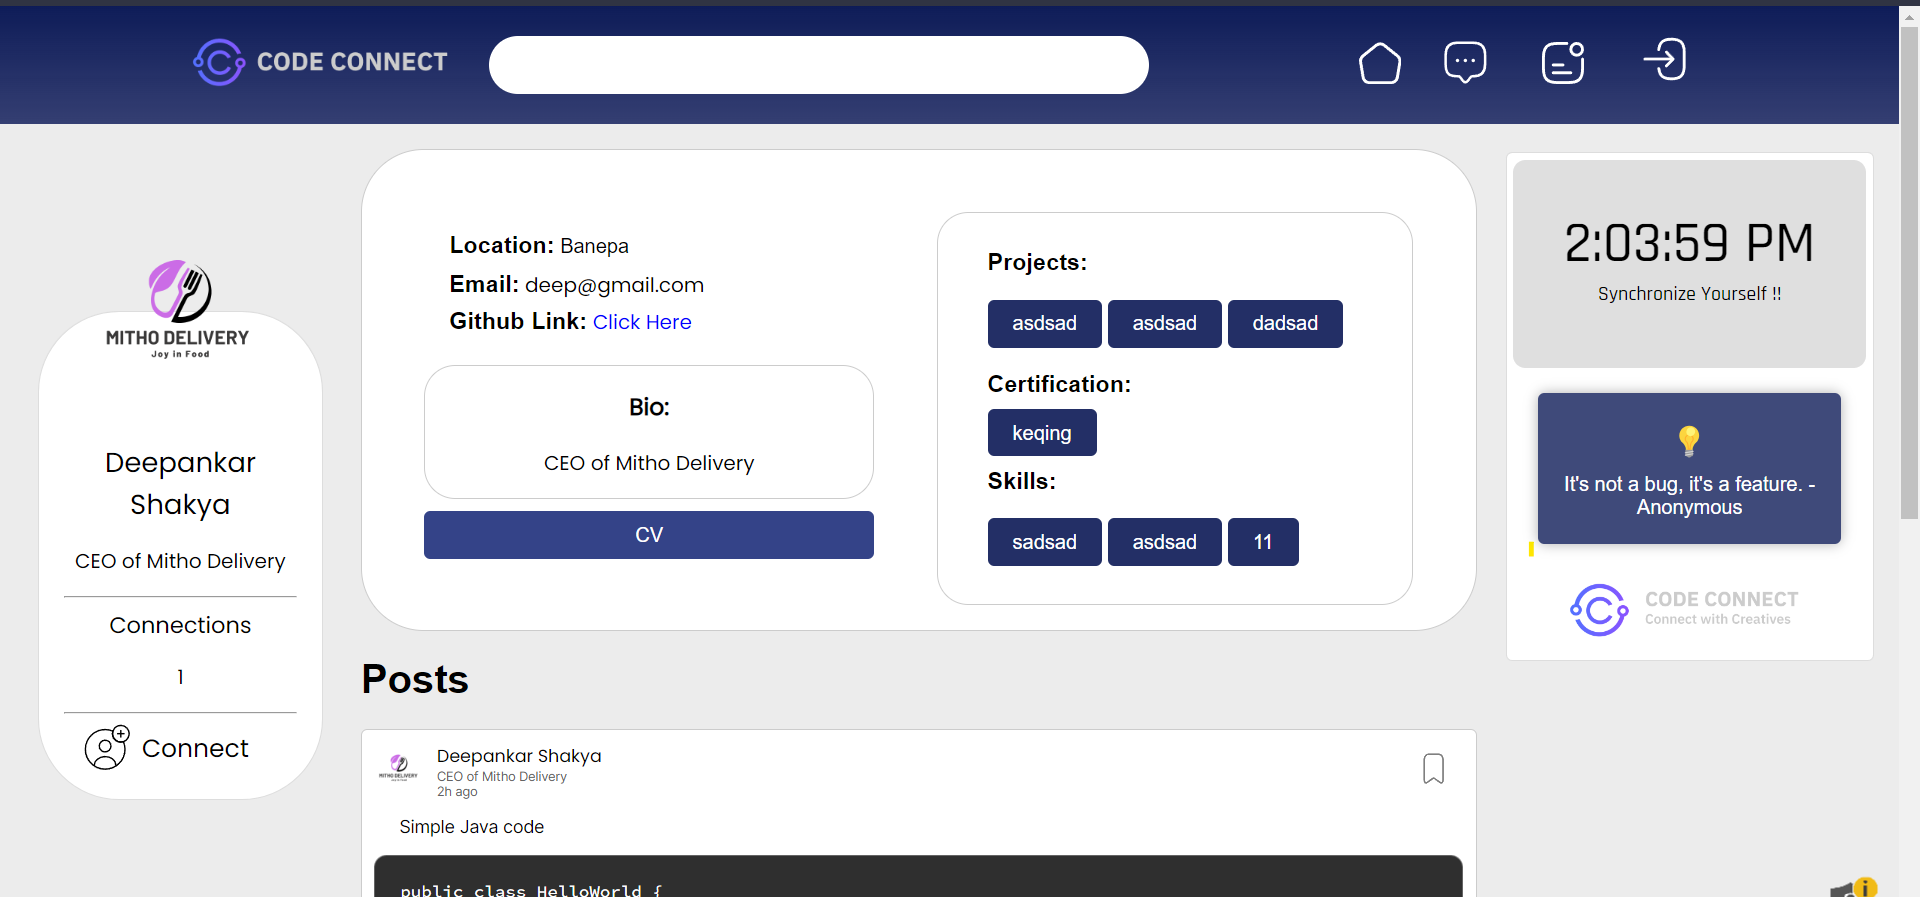
\includegraphics[width=1\textwidth]{Outcome-ss/other-user-profile.png}
    \caption{Profile of other Users.}
    \label{fig:Profile of other Users}
\end{figure}
\newpage
\subsection{Send Connection Request}
Sending a connection request is like asking someone if they want to be your friend on the platform. It's a way to show that you're interested in being connected and sharing things with them. If they accept, you can interact more and collaborate within the platform.
\begin{figure}[H]
    \centering
    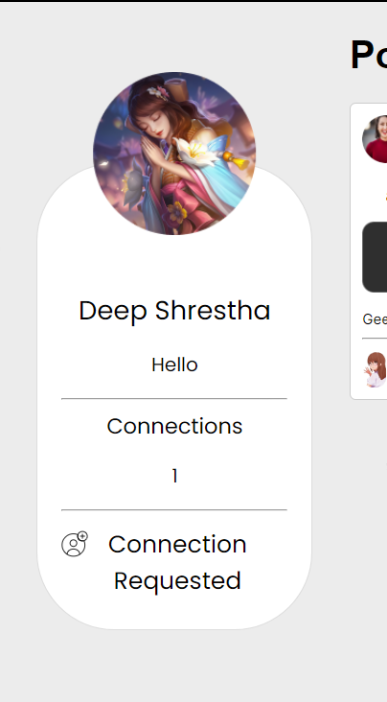
\includegraphics[height=0.3\textheight]{Outcome-ss/connection-request.png}
    \caption{Send Connection Request.}
    \label{fig:Send Connection Request}
\end{figure}
\subsection{Result after connection request is sent}
The image below gives you an idea of what it's like for another user when they receive a connection request. They'll see a notification that someone wants to connect with them. They can choose to accept the request and start connecting with the person who sent it. 
\begin{figure}[H]
    \centering
    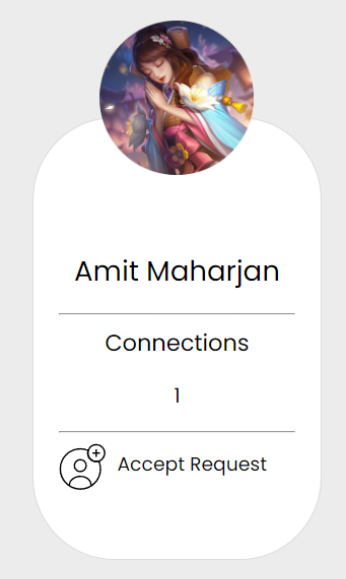
\includegraphics[height=0.3\textheight]{Outcome-ss/accept-request.png}
    \caption{Result after connection request is sent.}
    \label{fig:Result after connection request is sent}
\end{figure}
\subsection{Connection Request Accepted}
If the request is accepted, you'll see a "connected" sign, showing you're now friends. The person who sent the request will be added to your list of friends. This makes it easy to find and talk to each other, so you can work together and share stuff within the platform.
\begin{figure}[ht]
    \centering
    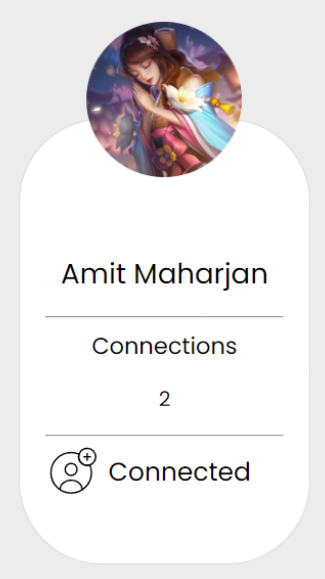
\includegraphics[height=0.3\textheight]{Outcome-ss/result-after-accepting.png}
    \caption{Connection Request Accepted.}
    \label{fig:Connection Request Accepted}
\end{figure}

\section{Conclusion}
In summary, "Code Connect" is a big step forward in creating a user-friendly social networking platform designed for IT professionals and developers. This report has explained the main features of the app, like posting discussions, Geeking, commenting, saving posts, managing profiles, and connecting with others. "Code Connect" is a helpful place where we can share knowledge, work together, and make new connections in the coding world. As we move ahead, how much we use it and enjoy it will show how successful it becomes in helping us learn, connect, and innovate in the tech field.

\section{Future Recommendations}

\chapter{DISCUSSION AND ANALYSIS}
Here,The platform offers a range of interactive features that promote collaboration, knowledge sharing, and connections among users. The home page serves as a user-friendly starting point, providing navigation options, announcements, and activity highlights. Users can express interest in content through the "Geek" feature and retract it using "Un-Geek." User profiles showcase activities and expertise, encouraging community building. The real-time messaging system facilitates instant communication and project discussions. A powerful search function suggests relevant user names for quick connections. Notifications keep users informed about updates, enhancing engagement. The "Post" feature allows content creation, sparking conversations and advice-sharing. Viewing profiles of other users fosters connections, and connection requests initiate networking. The platform's design promotes seamless interaction and meaningful engagement within the tech ecosystem, transforming "Code Connect" into a vibrant hub for industry professionals.
\\\\
The analysis of the "Code Connect" web application reveals a well-thought-out platform designed to cater to the specific needs of the tech community. The home page's user-centric layout is commendable, ensuring that users can seamlessly navigate and stay informed about recent activities. The incorporation of features like "Geek" and "Un-Geek" adds an element of user engagement and interactivity, akin to the familiar "like" and "dislike" mechanisms. User profiles offer a snapshot of individual presence, encouraging networking and collaboration by showcasing activities and expertise. The search functionality's dynamic suggestions enhance user experience by expediting connections. Notifications contribute to user engagement by ensuring timely updates. The "Post" feature not only allows content creation but also promotes knowledge sharing, further reinforcing the platform's collaborative ethos. Viewing profiles of other users and sending connection requests create a sense of community, while the visual representation of connection status facilitates networking.
% \chapter{WORKS REMAINING} 
% Below are the things which are need to be implemented in out system:
% \section{Comments}
% Comments sections in our poject is yet to be implemented. Comment section by creating another comment database will be implemented which will follow the instructions of our ER diagram.
% \section{Messeneger}
% Real-time messaging in our system yet need to implement which can be implemented using AJAX and creating new database messages which is yet to be implemented. It will be also implemented by the help of or ER diagram.
% \section{Search for Codes/Discussion}
% Search for user has been created but same logic for searching Discussion and Codes need to implemented. Button through which users can toggle between user search or Code/Discussion Search should be created.
% \section{CV Upload and Management}
% One of the most important tool need to be implemented through which users will be able to upload their CV and they will also have a section to shows the highlights of their CV
% \section{Portfolio management}
% This is also another core feature yet to be implemented in our system which showcases their projects with github links.
